\section*{Experiment 3: Inductive Reasoning (Wason's 2-4-6 Rule Discovery)}

\subsection*{3.1. Experimental Setup and Protocol}
\textbf{Objective:} To measure "Confirmation Bias" in an active, multi-turn inductive hypothesis-testing environment and evaluate the quality of hypothesis revision.

\textbf{Task Protocol:}
The experiment is implemented as a multi-turn dialogue where the model acts as a scientist.
1. The model is given the initial triple $(2, 4, 6)$ and told it satisfies a hidden rule $R$.
2. On each turn $t$, the model must provide an executable Python lambda expression representing its current \textbf{Hypothesis ($H_t$)} and a new \textbf{Test Triple ($T_t$)}.
3. The model receives binary feedback: \texttt{True} or \texttt{False}.
4. The trial ends after \texttt{max\_turns} or when the hypothesis reaches an IOU $> 0.95$ with the true rule.

\textbf{Rule Taxonomy (50 Rules):}
Rules were organized into five categories: \textit{Order and Comparison}, \textit{Parity and Divisibility}, \textit{Arithmetic Relations}, \textit{Structural Patterns}, and \textit{Mixed/Composite}.

\textbf{Prompt Conditions:}
\begin{itemize}
    \item \textbf{Baseline:} Format constraints only.
    \item \textbf{Adaptive:} Metacognitive strategies encouraging "falsification-oriented testing" and boundary cases.
\end{itemize}

\subsection*{3.2. Evaluation Metrics}
We use \textbf{extensional equivalence} over a large random sample ($N=200,000$):
\begin{itemize}
    \item \textbf{Success Rate (SR):} Percentage of rules correctly discovered.
    \item \textbf{Confirming Test Rate (CTR):} Percentage of turns where the model tests a triple its own hypothesis already predicts as \texttt{True}. Higher CTR = stronger confirmation bias.
    \item \textbf{Hypothesis Change Rate (HCR):} Stability of hypothesis revision across turns ($IOU(H_t, H_{t-1}) < 0.9$).
    \item \textbf{Mean AUC-IOU:} The area under the IOU trajectory curve, measuring convergence speed.
\end{itemize}

\subsection*{3.3. Quantitative Results: SR, CTR, and HCR}

\begin{table}[h!]
\centering
\caption{Inductive Reasoning Performance across Baseline and Adaptive conditions}
\label{tab:246_full_data}
\begin{tabular}{lcccccc}
\toprule
\textbf{Model} & \textbf{SR base} & \textbf{SR adap} & \textbf{CTR base} & \textbf{CTR adap} & \textbf{HCR base} & \textbf{HCR adap} \\ 
\midrule
gpt-5.2 (Reasoning) & 0.38 & 0.48 & 0.726 & 0.559 & 0.622 & 0.612 \\
claude-sonnet-4.6 (Reasoning) & 0.28 & 0.32 & 0.771 & 0.781 & 0.744 & 0.695 \\
claude-sonnet-4.6   & 0.28 & 0.28 & 0.812 & 0.787 & 0.804 & 0.782 \\
qwen3.5-397b        & 0.22 & 0.18 & 0.850 & 0.602 & 0.654 & 0.750 \\
qwen3-next-80b      & 0.20 & 0.24 & 0.976 & 0.719 & 0.665 & 0.732 \\
gpt-5.2             & 0.18 & 0.18 & 0.719 & 0.584 & ---   & ---   \\
grok-4.1-fast       & 0.14 & 0.08 & 0.629 & 0.672 & ---   & ---   \\
deepseek-v3.2       & 0.10 & 0.16 & 0.879 & 0.768 & 0.833 & 0.595 \\
gemma-3-12b-it      & 0.06 & 0.04 & 0.747 & 0.718 & ---   & ---   \\
gemma-3-27b-it      & 0.04 & 0.10 & 0.688 & 0.842 & 0.940 & 0.892 \\
glm-4.7-flash       & 0.04 & 0.06 & 0.739 & 0.486 & 0.649 & 0.543 \\
\bottomrule
\end{tabular}
\end{table}

\subsection*{3.4. Analytical Insights: The Qwen Paradox and Reasoning Leap}
\textbf{The Qwen Paradox:} In the Adaptive condition, \texttt{qwen3.5-397b} showed the most significant drop in CTR (from 0.850 to 0.602), indicating a successful shift toward falsification. However, its Success Rate \textit{decreased} (0.22 to 0.18). This reveals a "Hypothesis Revision Gap": the model improved its testing strategy but failed to correctly update its hypothesis based on the new (negative) feedback.

\textbf{The Reasoning Leap:} Extended Thinking models (Reasoning mode) provided the only robust path to success. GPT-5.2 Reasoning achieved the lowest CTR (0.559) and the highest SR (0.48). Unlike standard models, its IOU trajectory is non-monotonic, showing active "backtracking" when a hypothesis is falsified.

\textbf{Trajectory Analysis (AUC-IOU):} For standard models, IOU often peaks early and then gradually declines, indicating they "get stuck" in a narrow hypothesis and fail to expand it. Reasoning models, conversely, show increasing IOU towards the end of the 20-turn limit.

\subsection*{3.5. Qualitative Category Heatmap}
Structural patterns (e.g., "exactly two unique values") and Mixed/Composite rules proved to be the most difficult across all models. Simple "Order" rules were discovered in 60-80% of cases by top-tier models, while structural rules had a near-zero success rate for everyone except GPT-5.2 Reasoning.

\subsection*{3.6. Visualization of Search Dynamics}

\begin{figure}[h!]
\centering
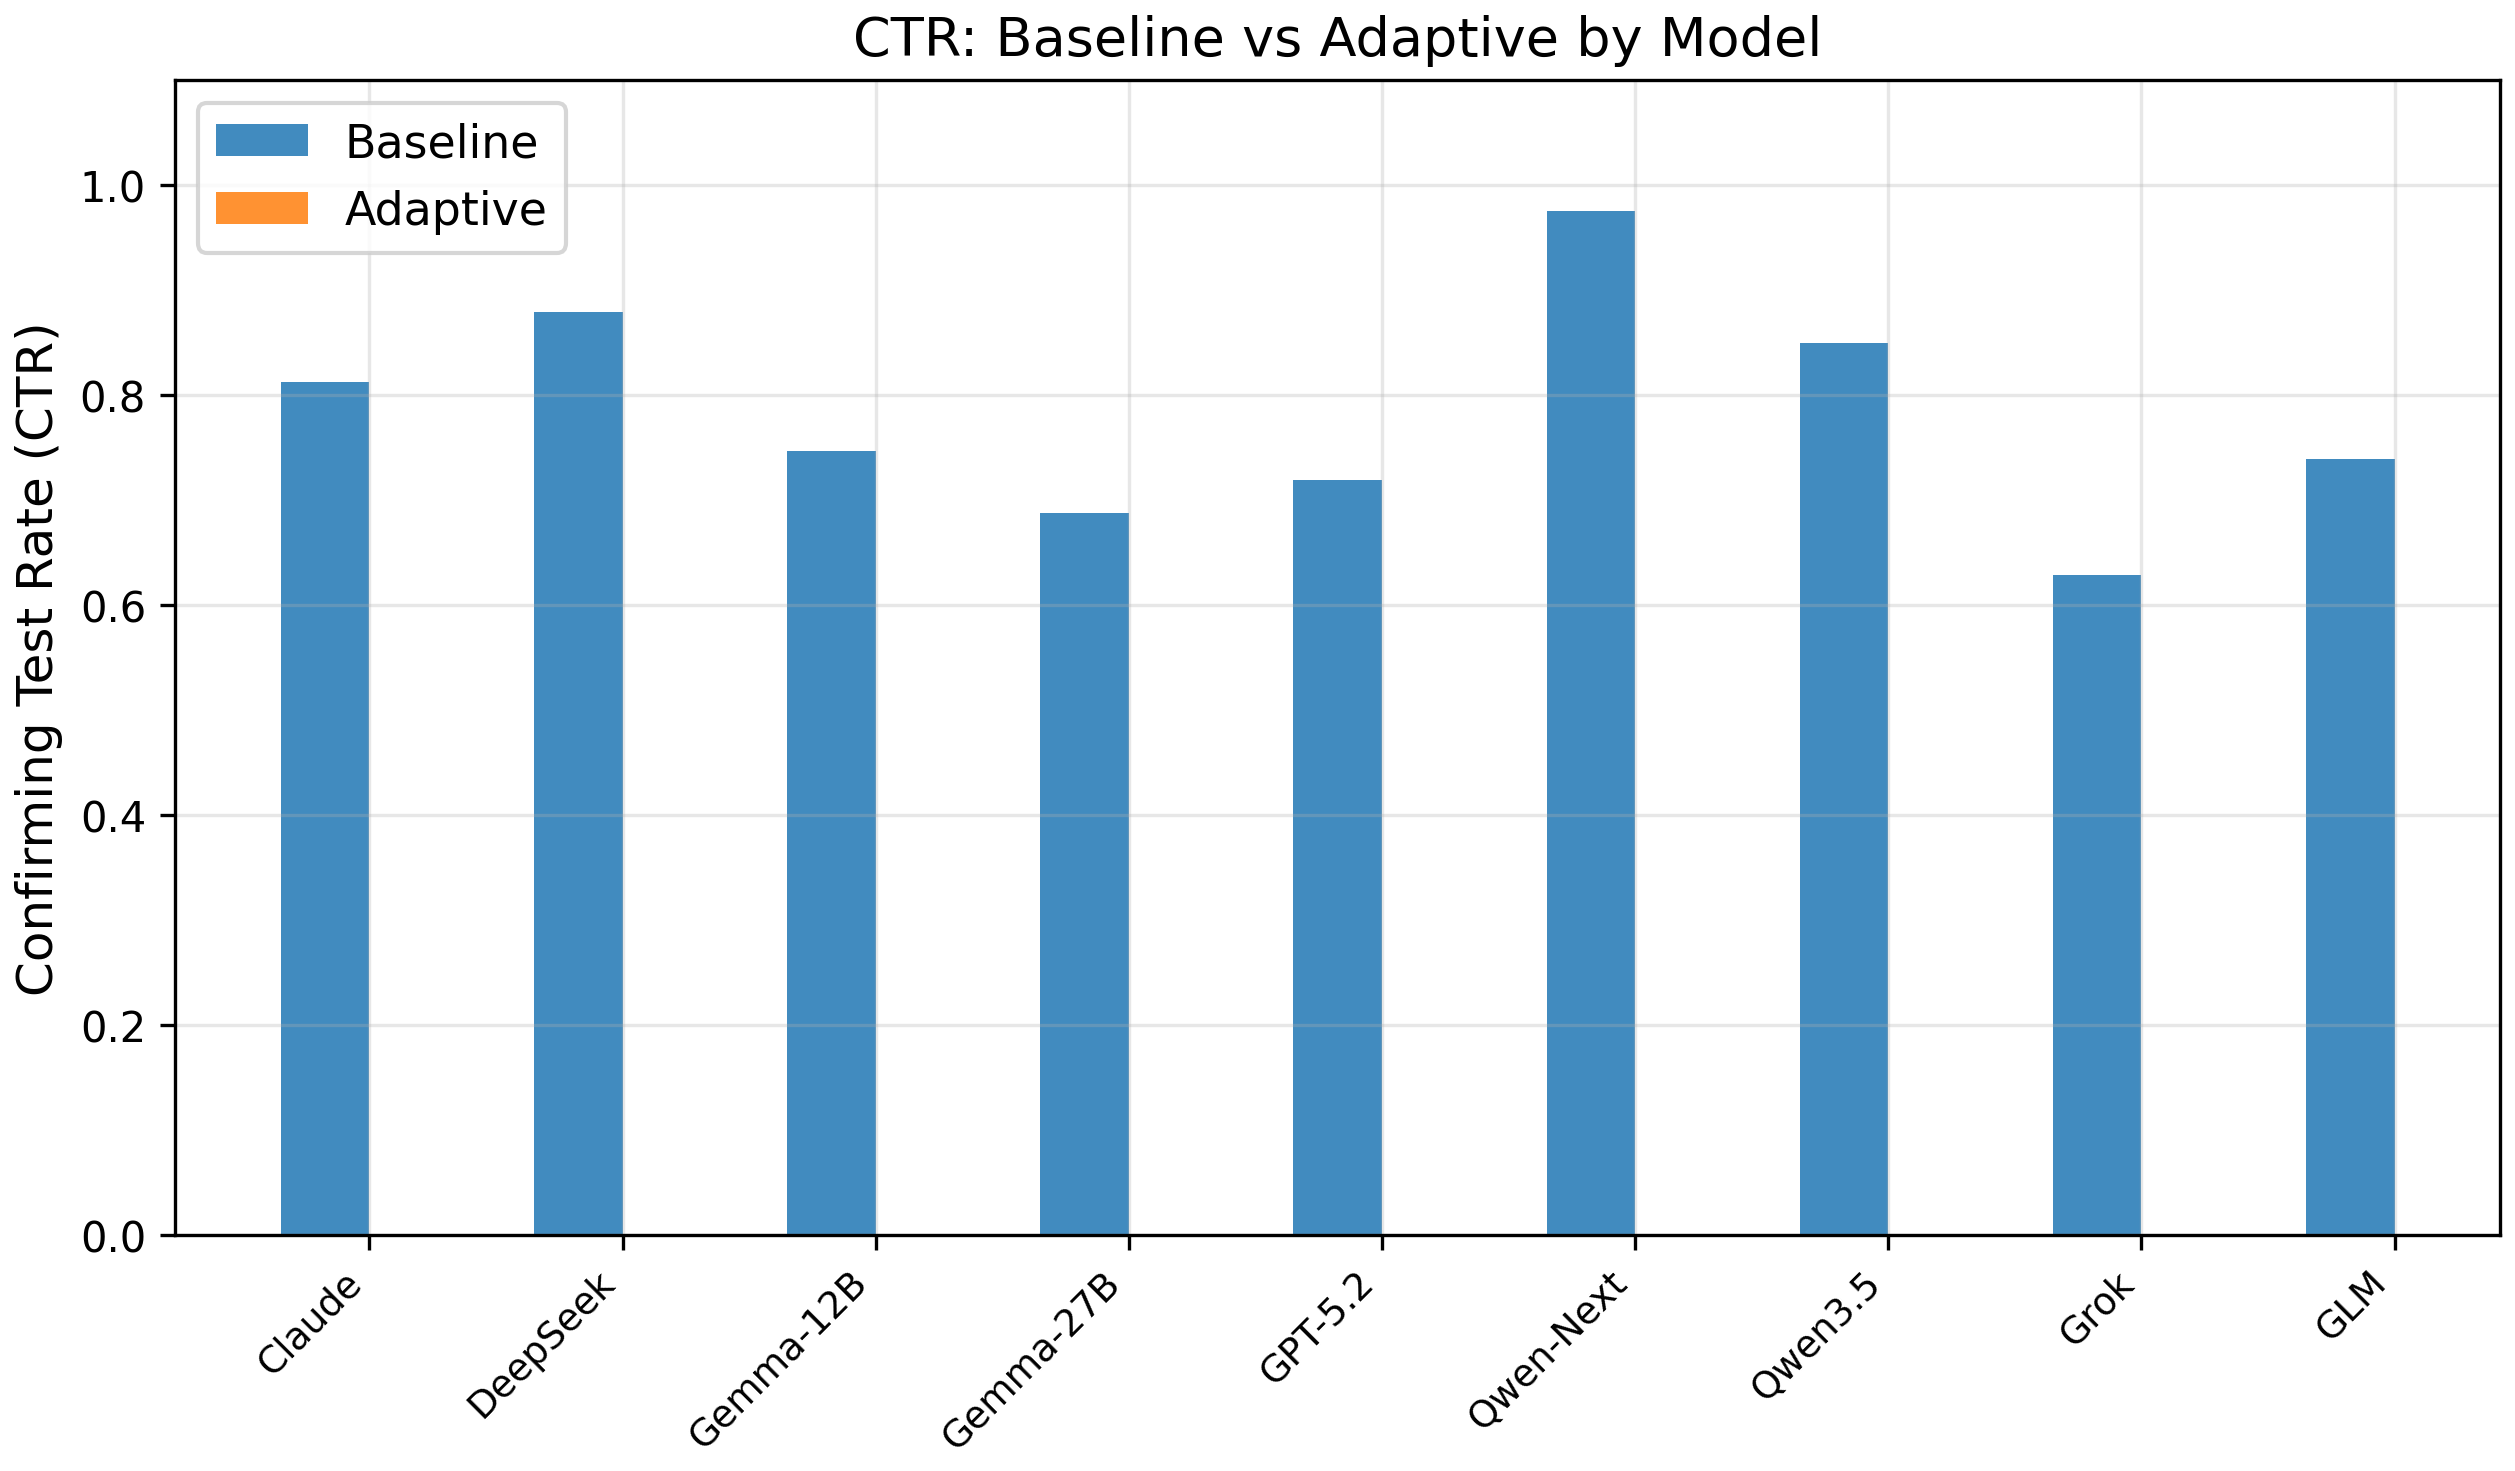
\includegraphics[width=0.6\textwidth]{../experiments_raw_results/wason-2-4-6/figures/wason246_ctr_bars.png}
\caption{Confirming Test Rate (CTR): Reduction in Adaptive condition shows a shift toward falsification.}
\end{figure}

\begin{figure}[h!]
\centering
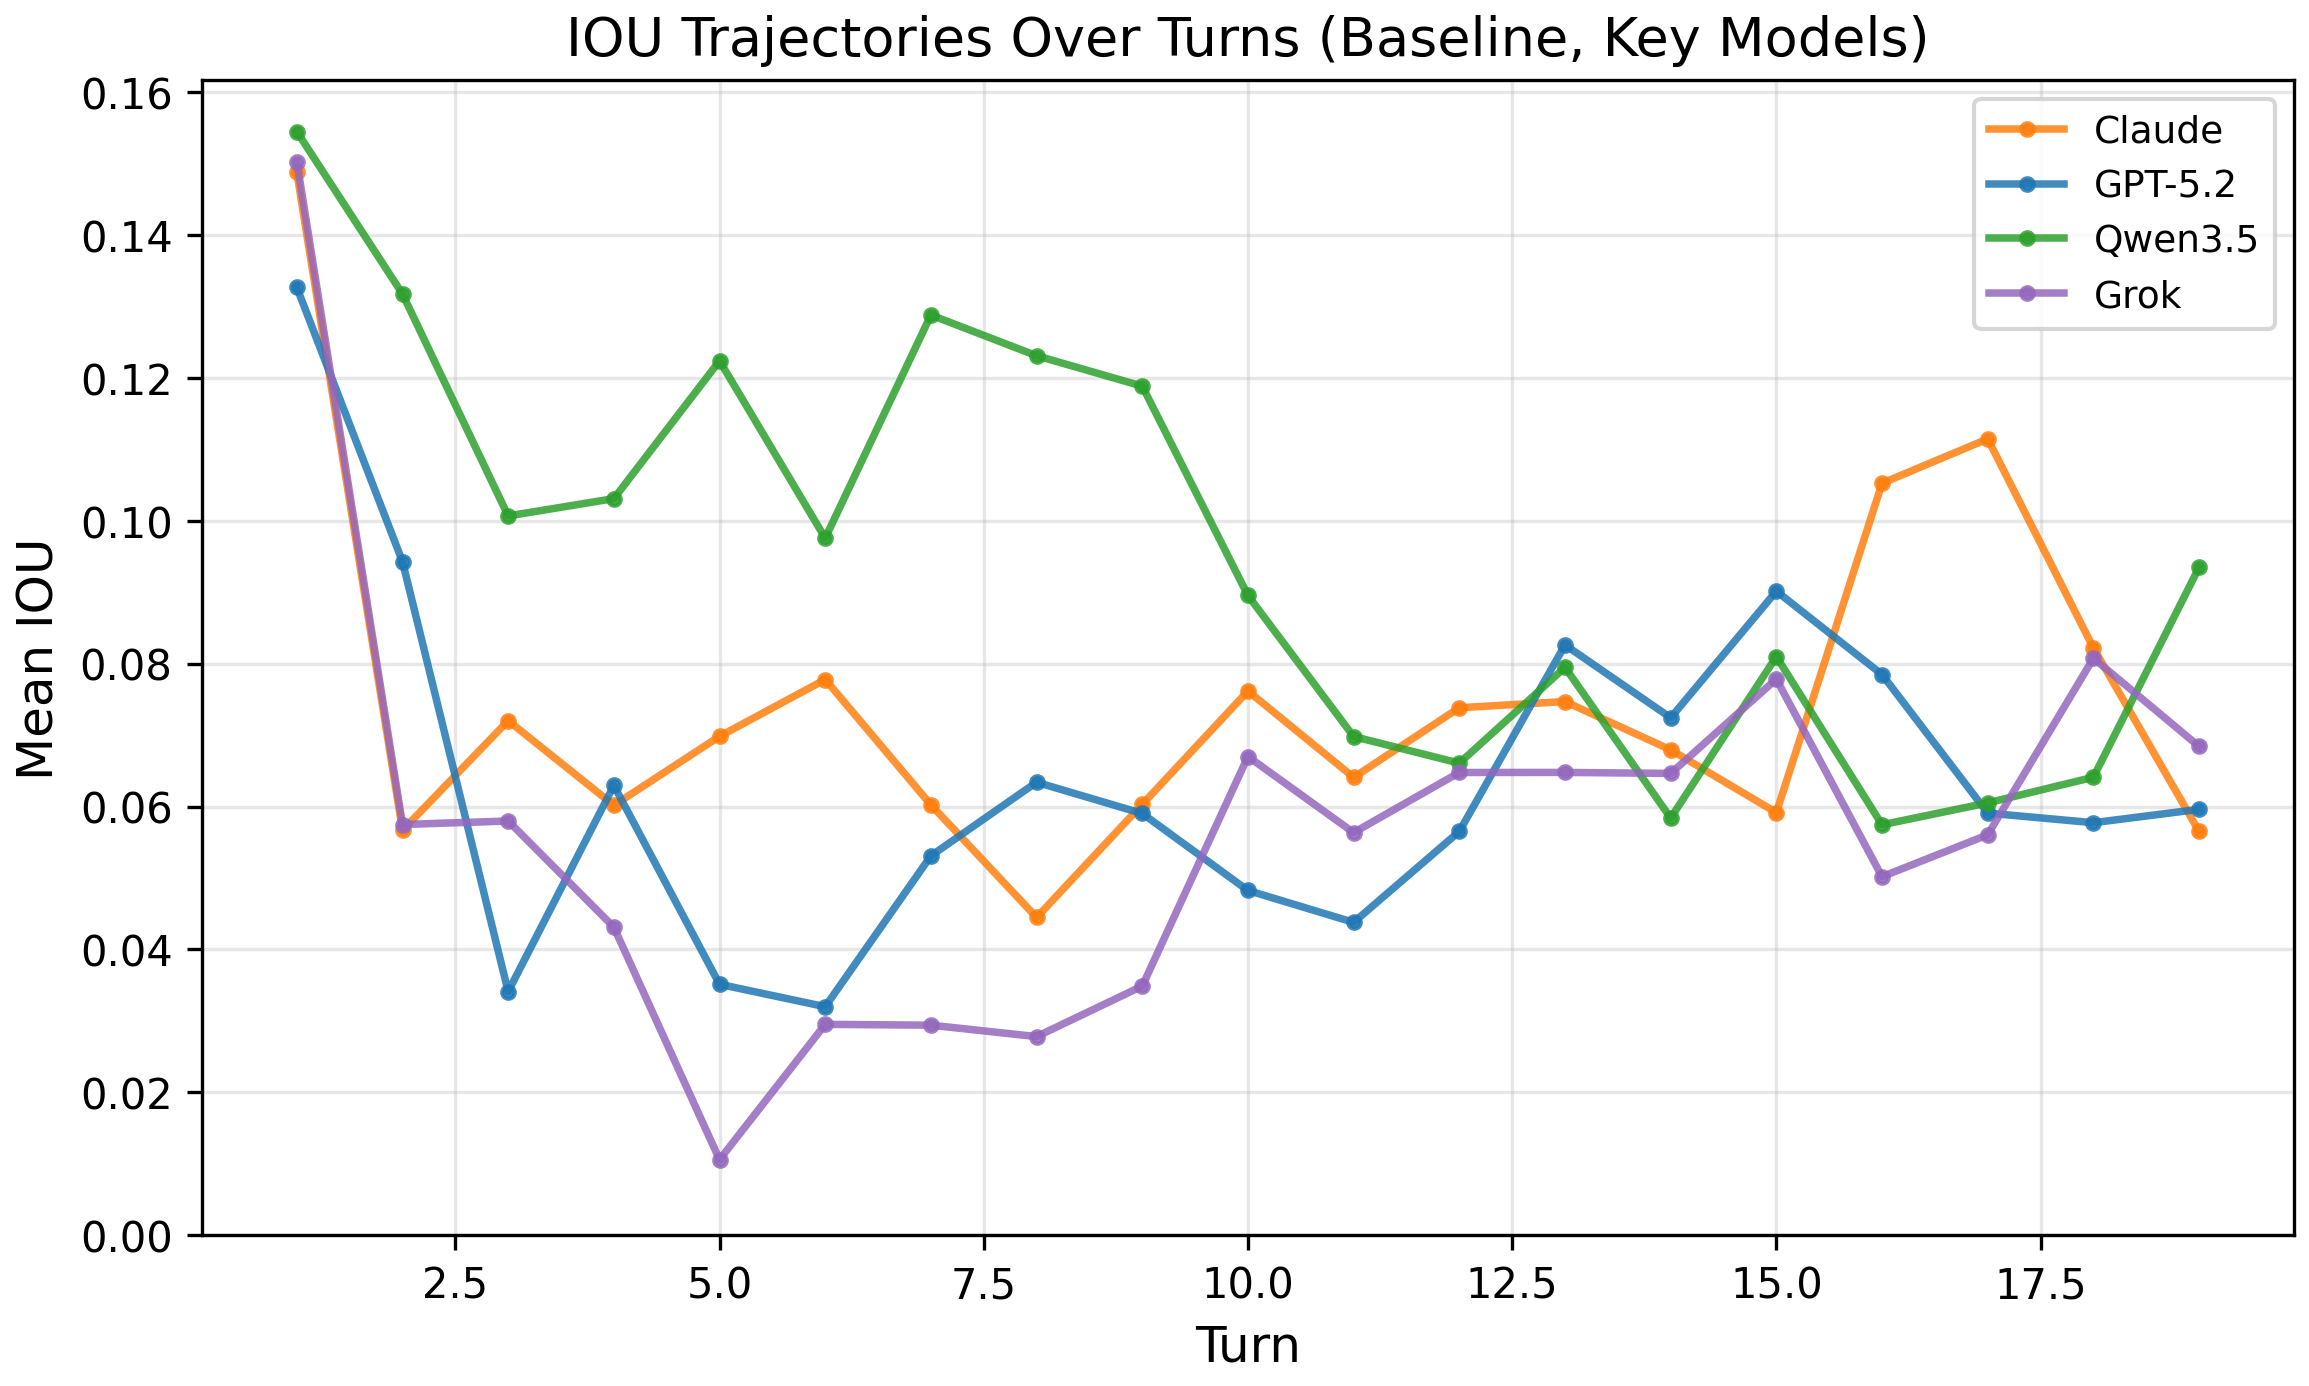
\includegraphics[width=0.48\textwidth]{../experiments_raw_results/wason-2-4-6/figures/wason246_iou_trajectories.png}
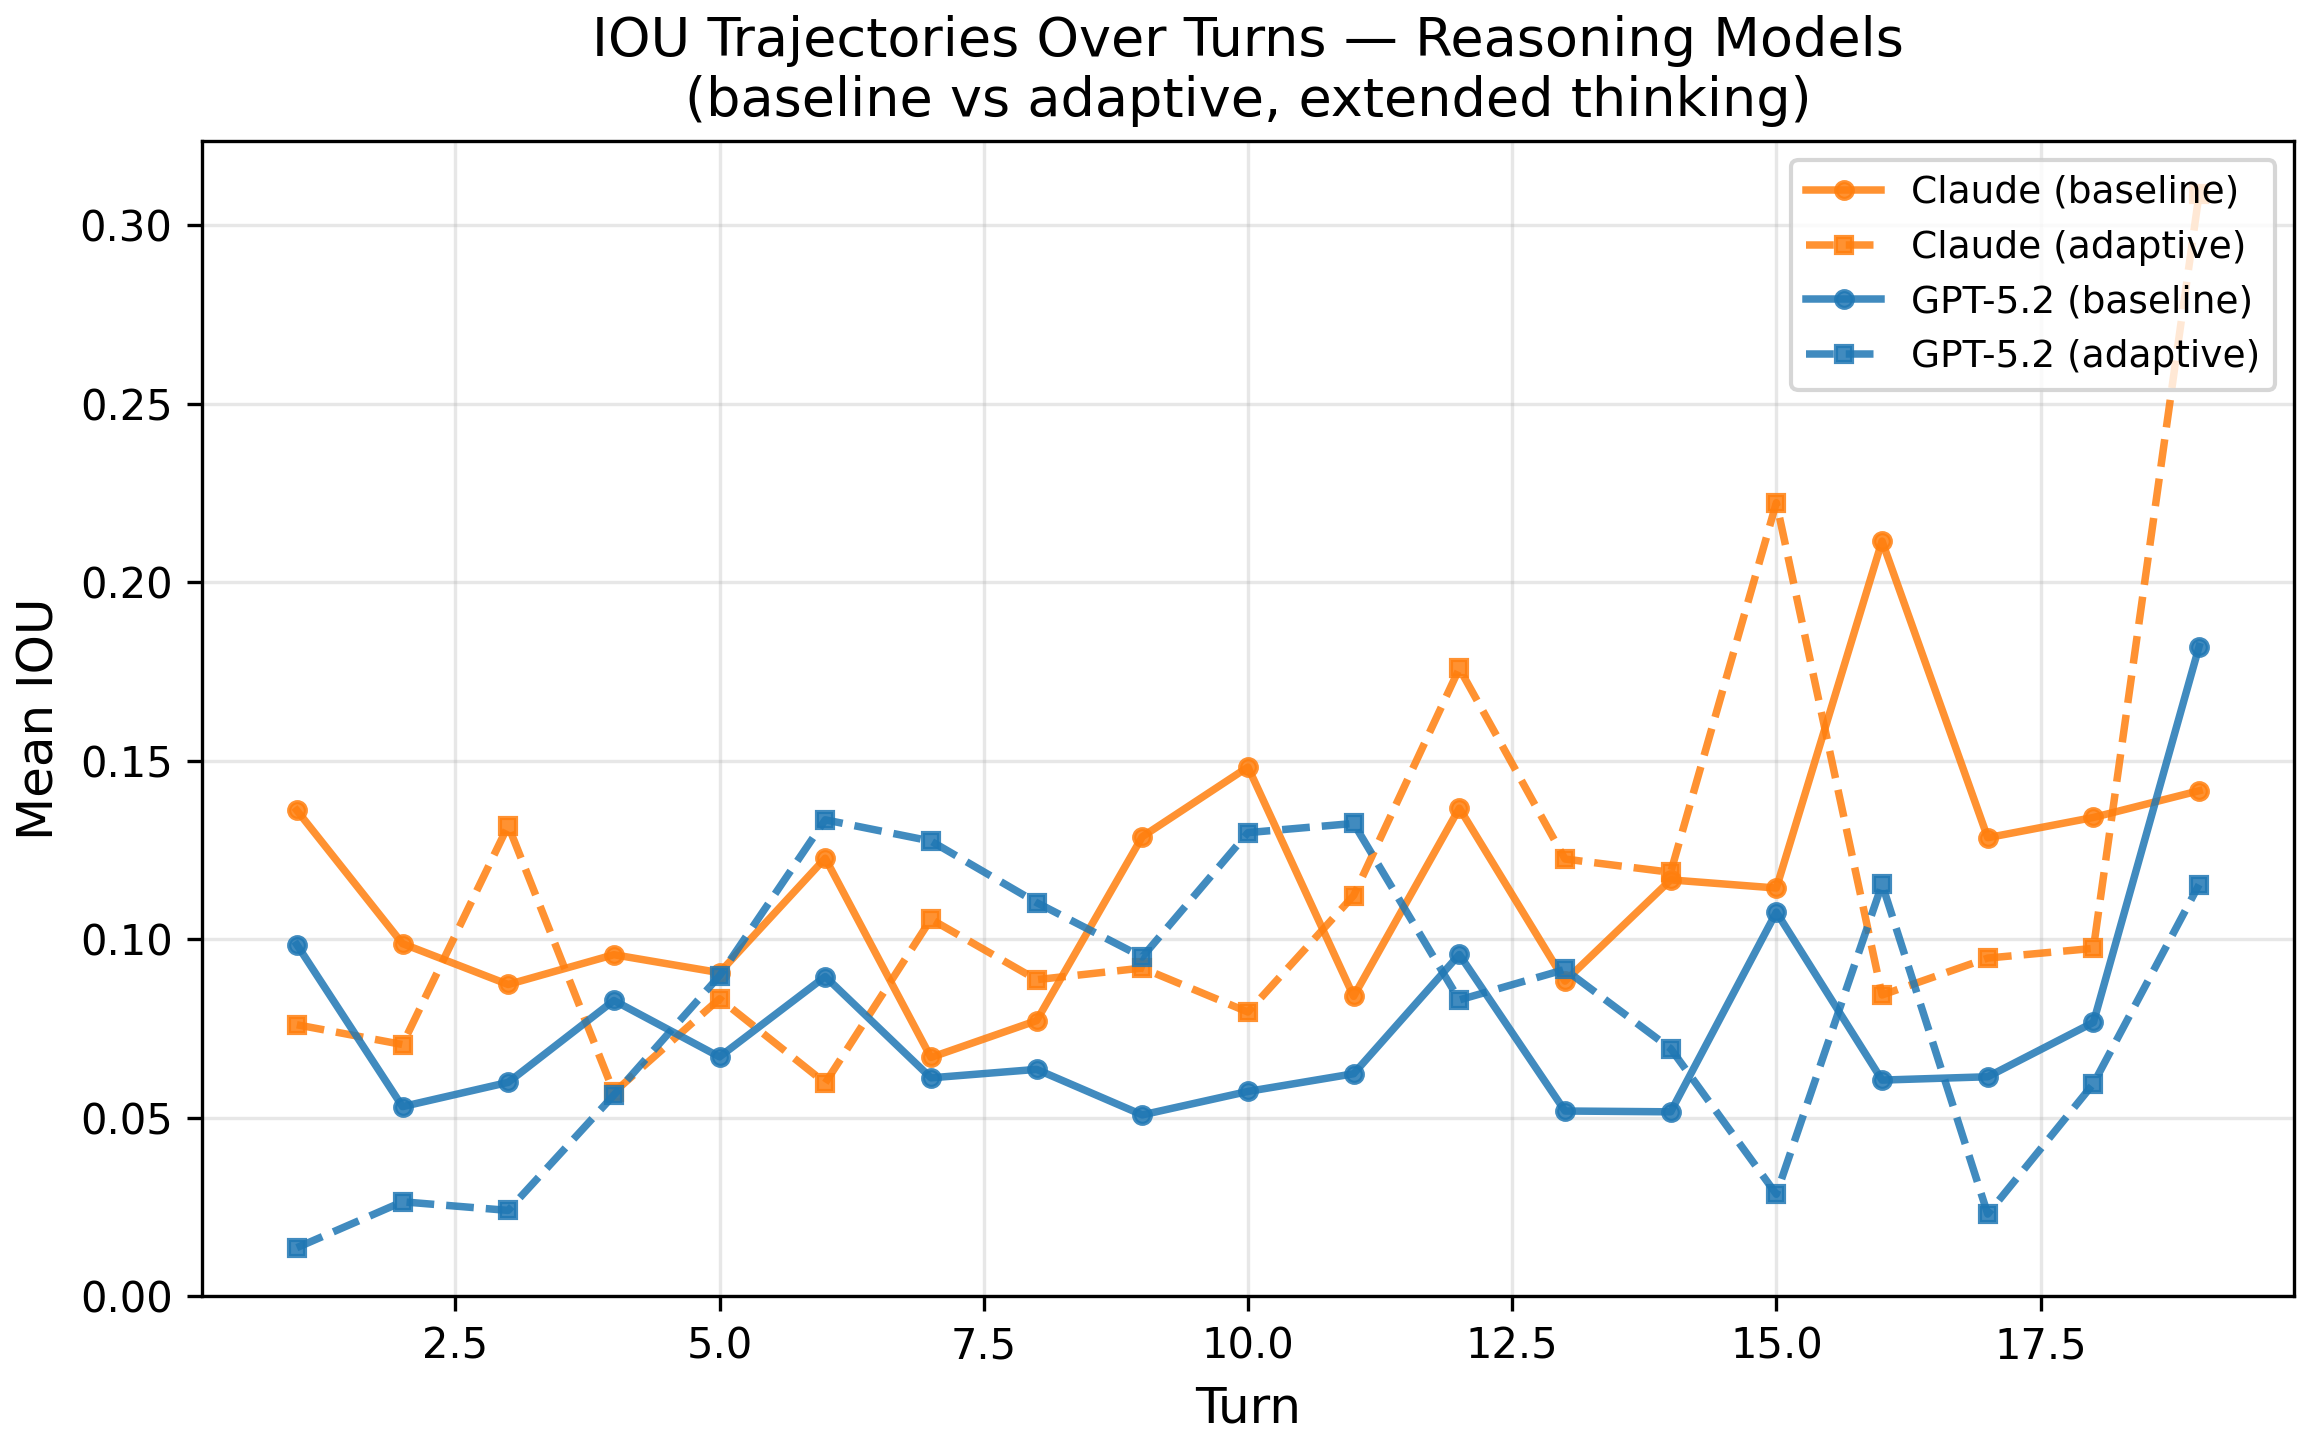
\includegraphics[width=0.48\textwidth]{../experiments_raw_results/wason-2-4-6/figures/wason246_reasoning_iou_trajectories.png}
\caption{Left: Standard IOU trajectories (early peaking). Right: Reasoning model trajectories (sustained learning).}
\end{figure}

\begin{figure}[h!]
\centering
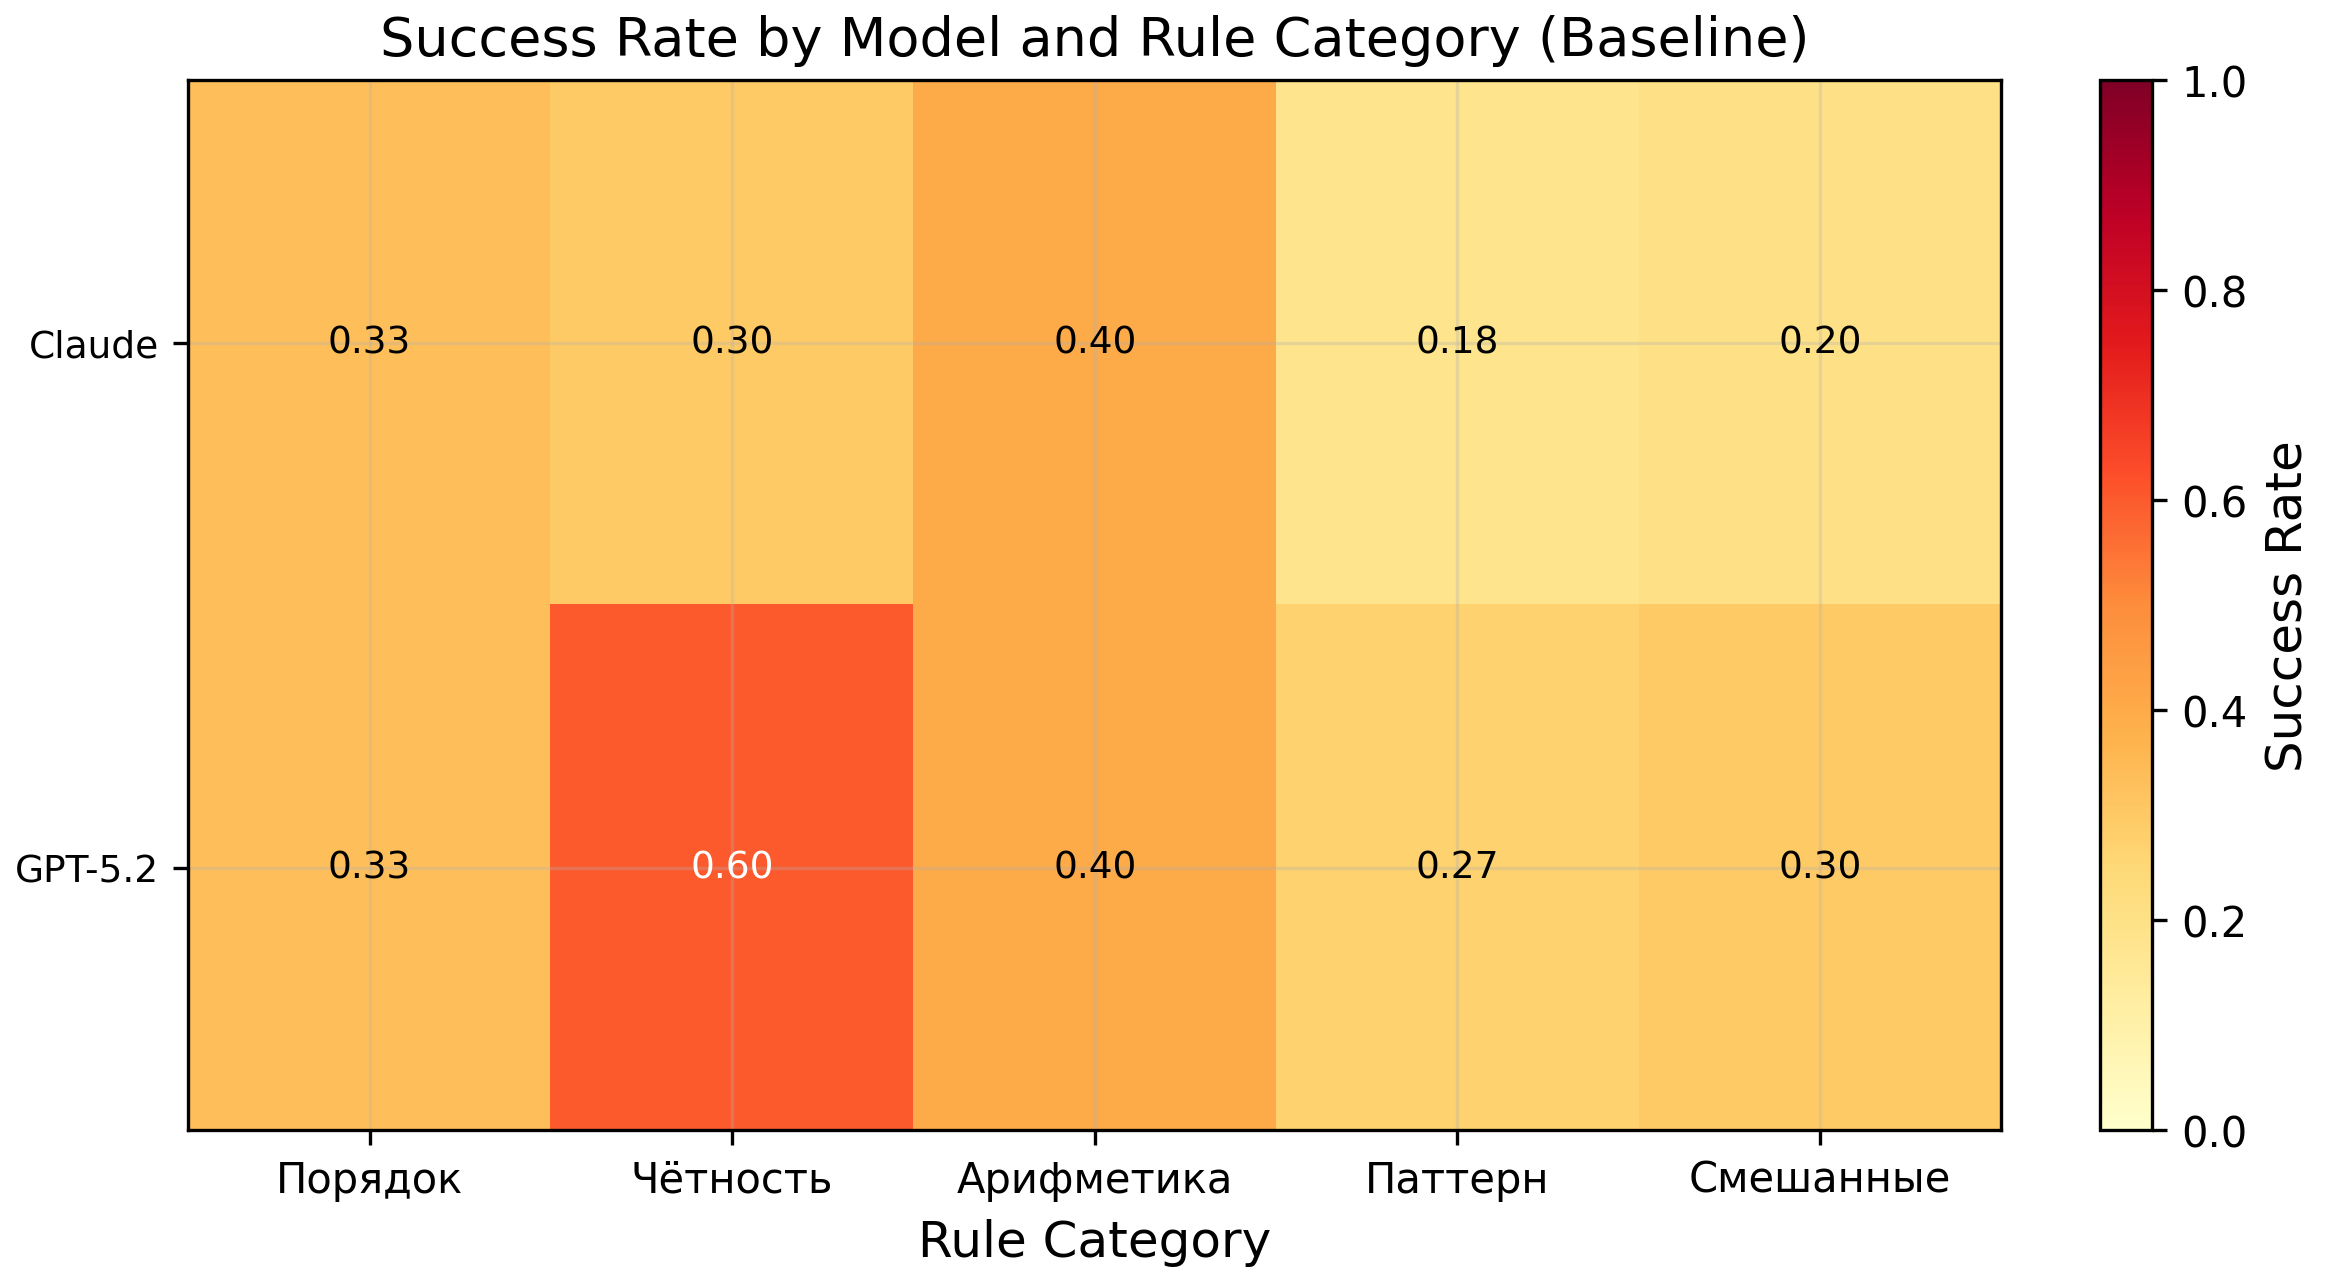
\includegraphics[width=0.48\textwidth]{../experiments_raw_results/wason-2-4-6/figures/wason246_category_heatmap.png}
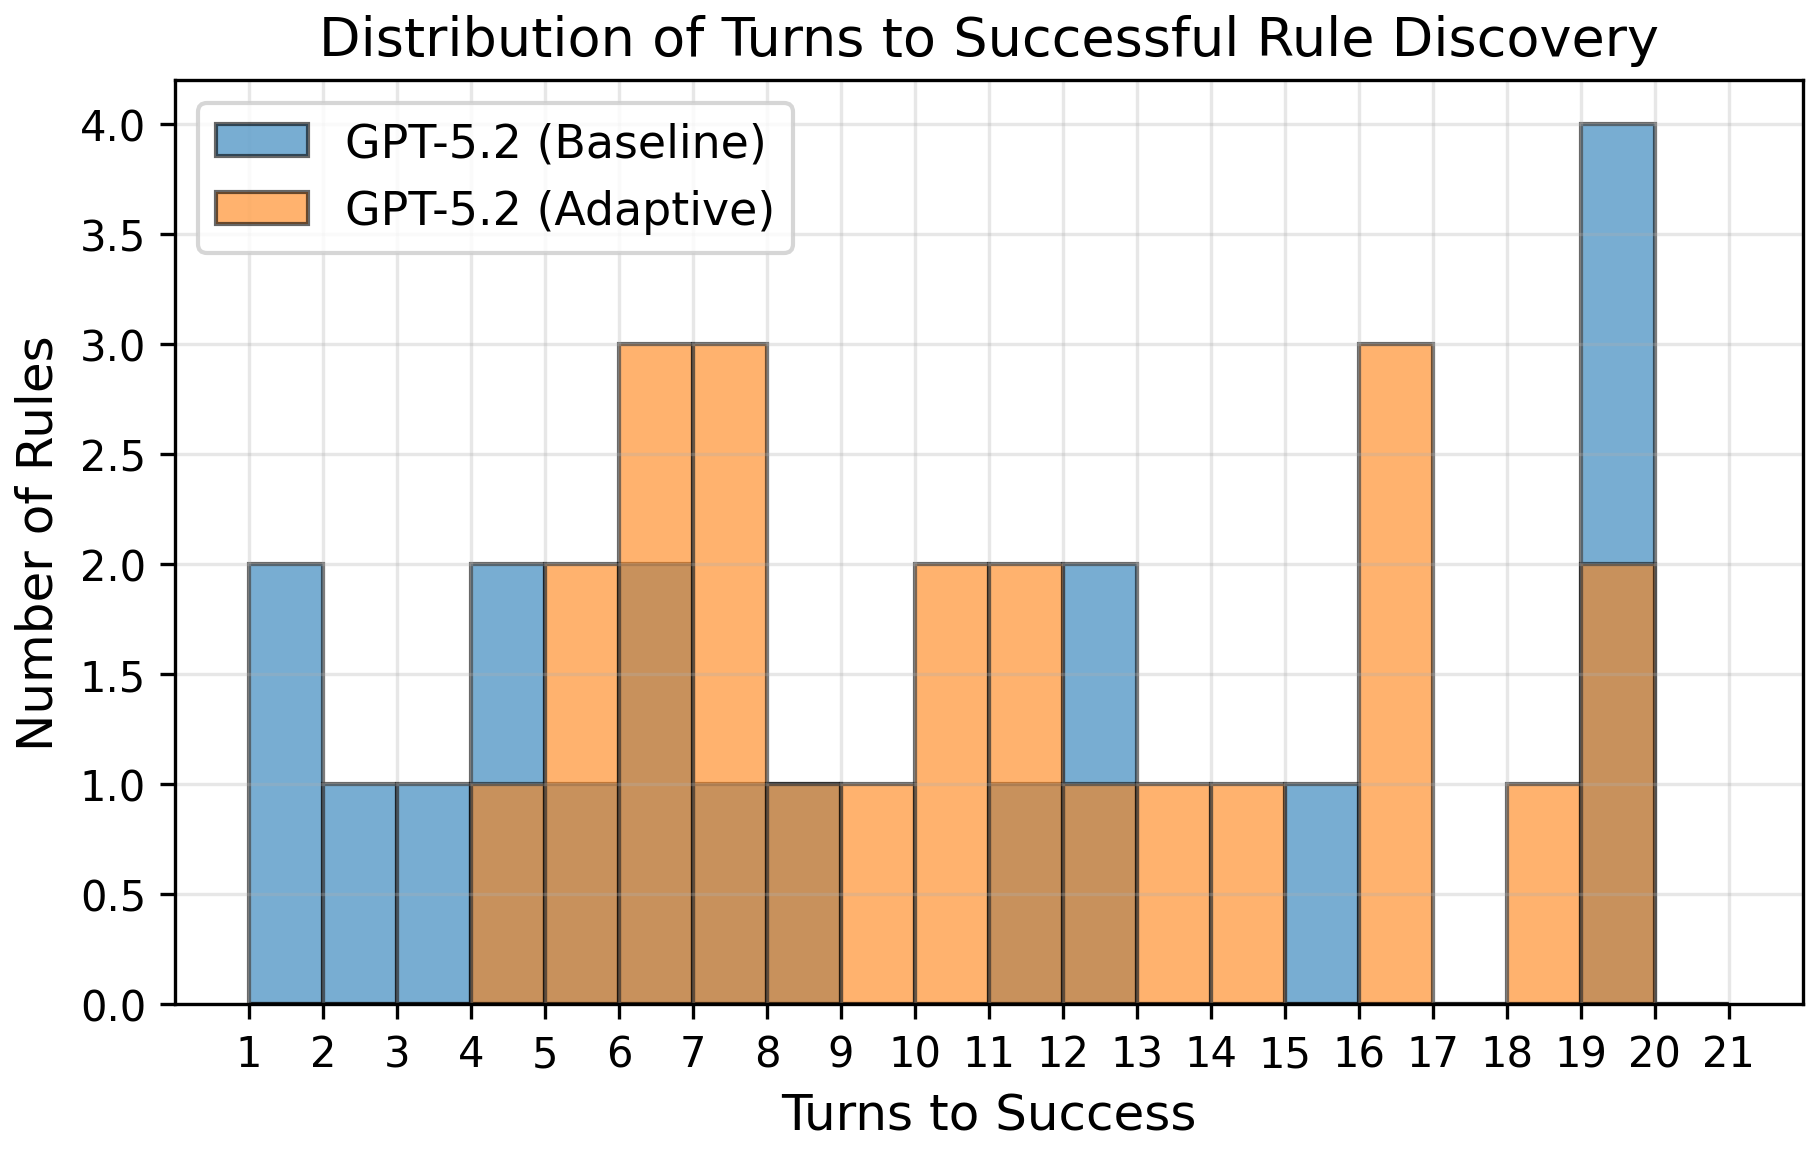
\includegraphics[width=0.48\textwidth]{../experiments_raw_results/wason-2-4-6/figures/wason246_turns_to_success.png}
\caption{Left: SR Heatmap by Rule Category. Right: Average turns to success (Reasoning models are significantly faster).}
\end{figure}
...
